\section{God Of War III}

\begin{figure}[htbp]
\begin{center}
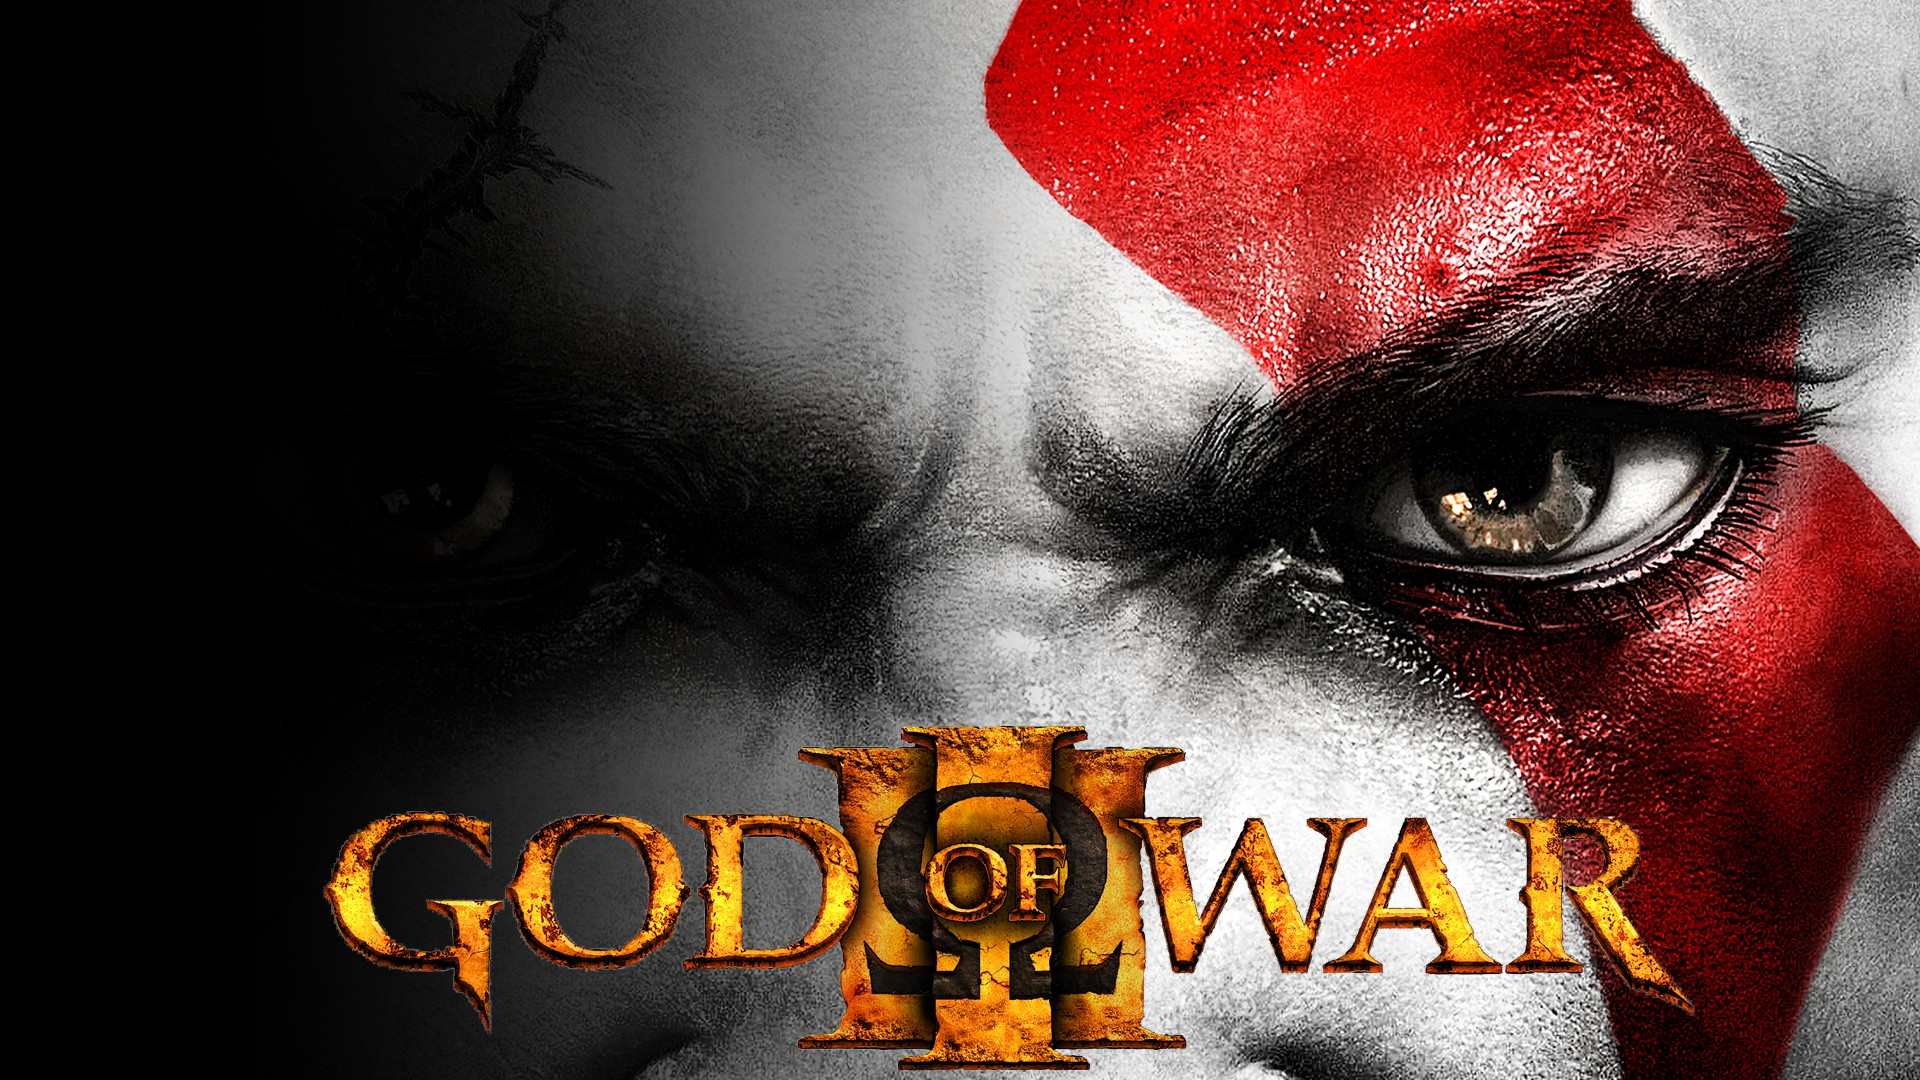
\includegraphics[width=.60\textwidth]{./imagenes/godofwar3.jpg}
\caption{God Of War III}
\label{God Of War III}
\end{center}
\end{figure}
God Of War III\footnote{\url{http://www.ign.com/games/god-of-war-iii/ps3-886158/}} God of War III es un juego basado en la mitologia griega, en donde el personaje principal llamado Kratos, el cual era el antiguo Dios de la Guerra, asciende al olimpo con la ayuda de los Titanes para tomar venganza de Zeus ya que éste lo habia traicionado. Ya en el olimipo se enfrentara a todos los dioses que habitan ahi, incluidos los tres mas poderosos Hades, Poseidon y por ultimo Zeus, pero Kratos estara ayudado por Atenea quien lo guiará a lo largo del juego y le dara la clave para poder derrotar a Zeus. 

\subsubsection{¿Por qué es uno de mis juegos favoritos?}
\begin{itemize}
\item[Kevin Silva] El juego es muy real, ha sido premiado por la calidad de graficos y su trama es muy envolvente. Tambien posee minijuegos de logica a lo largo que vas avanzando por el juego. El juego no es muy corto pero tampoco muy extenso y en el camino podras encontrarte con muchos enemigos, tambien poder controlar un sinnumero de armas conforme vayas ganado batallas y a la vez escoger cual de ellas aumentarles de poder. En fin el juego te da muchas posibilidades y brinda garantia de que no te aburrirás al jugarlos, es por ésta razon que fue catalogado como el "Videojuego mas esperado del 2010"  
\end{itemize}
